\iffalse
\documentclass[12pt]{article}
\usepackage{graphicx}
\usepackage{amsmath}
\usepackage{mathtools}
\usepackage{gensymb}
\usepackage{tabularx}
\usepackage{array}
\usepackage[latin1]{inputenc}
\usepackage{fullpage}
\usepackage{color}
\usepackage{array}
\usepackage{longtable}
\usepackage{calc}
\usepackage{multirow}
\usepackage{hhline}
\usepackage{ifthen}
\usepackage{lscape}
\usepackage{float}
\usepackage{amssymb}

\newcommand{\mydet}[1]{\ensuremath{\begin{vmatrix}#1\end{vmatrix}}}
\providecommand{\brak}[1]{\ensuremath{\left(#1\right)}}
\providecommand{\norm}[1]{\left\lVert#1\right\rVert}
\providecommand{\abs}[1]{\left\vert#1\right\vert}
\newcommand{\solution}{\noindent \textbf{Solution: }}
\newcommand{\myvec}[1]{\ensuremath{\begin{pmatrix}#1\end{pmatrix}}}
\let\vec\mathbf

\def\inputGnumericTable{}

\begin{document}
\begin{center}
\textbf\large{OPTIMIZATION}

\end{center}
\section*{Excercise 6.6}


\solution
\fi
The given equation of the curve can be written as  
\begin{align}
	\label{eq:12/6/6/4/conv/parabolaEq2}
	g\brak{\vec{x}} = \vec{x}^\top\vec{V}\vec{x} + 2\vec{u}^\top\vec{x} + f = 0 
\end{align}
where
\begin{align}
	\vec{V} = \myvec{ 1 & 0 \\ 0 & 0} ,\,
	\vec{u} = \myvec{0 \\ -2} ,\,
	f = 0 
\end{align}
We are given that 
\begin{align}
	\vec{P} &= \myvec{4 \\ -2}
\end{align}
This can be formulated as optimization problem as follows:
\begin{align}
	\label{eq:12/6/6/4/conv/Eq3}
	&  \min_{\vec{x}} \quad \text{g}\brak{\vec{x}} = \norm{\vec{x}-\vec{P}}^2\\
	\label{eq:12/6/6/4/conv/Eq4}
	& \text{s.t.}\quad h\brak{\vec{x}} = \vec{x}^\top\vec{V}\vec{x} + 2\vec{u}^\top\vec{x} + f = 0  
\end{align}
From 
	    \ref{app:quad-nonconv}, the
given problem is not convex. Hence, using the relaxation (see 
	    \ref{app:quad-conv})
\begin{align}
	\label{eq:12/6/6/4/conv/Eq7}
	& g\brak{\vec{x}} = \vec{x}^\top\vec{V}\vec{x} + 2\vec{u}^\top\vec{x} + f \le 0  
\end{align}
the optimization problem can be made convex.  Solving the problem using \textit{cvxpy} we get 
\begin{align}
	\vec{x} = \myvec{1.695\\0.718}
\end{align}
See Fig. \ref{fig:12/6/6/4/conv/Fig1}.
\begin{figure}[!h]
	\begin{center} 
	    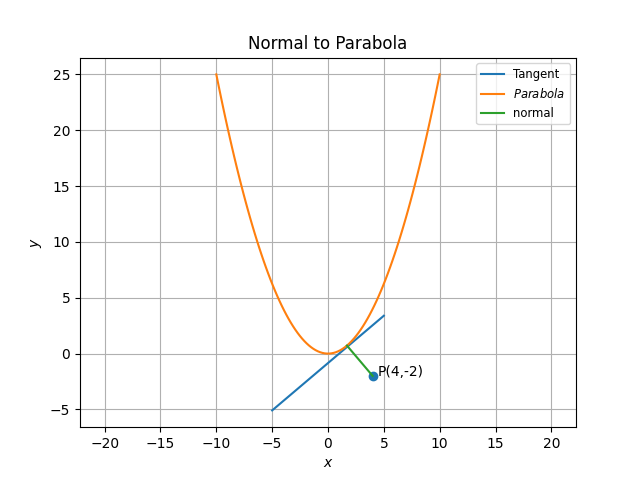
\includegraphics[width=\columnwidth]{12/6/6/4/conv/figs/12_6_6_4}
	\end{center}
\caption{}
\label{fig:12/6/6/4/conv/Fig1}
\end{figure}

